\documentclass[11pt]{article}
\usepackage{../../latex/stat4ml_style}

\title{Chapter 5: Convergence Concepts \\ \large Part I --- Statistics Foundation for ML}
\author{Omid Safarzadeh}
\date{}

\begin{document}
\maketitle

\begin{abstract}
\noindent
A single estimate is one number; what makes statistics possible is knowing
what happens to that number as the data pile up. This chapter is about the
limits of random quantities. Two results carry most of the weight: the
\emph{law of large numbers}, which says the sample mean converges to the true
mean, and the \emph{central limit theorem}, which says the error of that
sample mean is normal almost regardless of where the data came from. Together
they are why an average is trustworthy and why the normal distribution turns
up everywhere. We state them, watch them happen in code, prove them from two
elementary inequalities, and close with the handful of tools --- Slutsky's
theorem, the continuous mapping theorem, the delta method --- that the rest
of the course quietly relies on.
\end{abstract}

\tableofcontents

% ======================================================================
\section{The law of large numbers and the central limit theorem}
% ======================================================================

Let $X_1, X_2, \dots$ be independent and identically distributed, with mean
$\mu = E[X_i]$ and finite variance $\sigma^2 = \operatorname{Var}(X_i)$. The
object we care about is the \keyterm{sample mean}
$\bar X_n = \frac1n \sum_{i=1}^n X_i$. Its own mean and variance follow from
linearity:
\[
  E[\bar X_n] = \mu, \qquad \operatorname{Var}(\bar X_n) = \frac{\sigma^2}{n}.
\]
The mean stays put while the variance shrinks like $1/n$, so the distribution
of $\bar X_n$ should pile up tighter and tighter around $\mu$. Making
``piles up around'' precise is what a mode of convergence is for.

\begin{definition}[Convergence in probability]
A sequence $Y_n$ \emph{converges in probability} to $Y$, written
$Y_n \xrightarrow{p} Y$, if for every $\varepsilon > 0$,
\[
  P\big(|Y_n - Y| > \varepsilon\big) \longrightarrow 0 \quad\text{as } n\to\infty.
\]
\end{definition}

\begin{theorem}[Weak law of large numbers]
If $X_1,\dots,X_n$ are iid with mean $\mu$ and finite variance, then
$\bar X_n \xrightarrow{p} \mu$.
\end{theorem}

The law of large numbers is the guarantee that estimation works at all:
collect enough data and the sample mean is as close to the truth as you like.
But it says nothing about \emph{how} close, or about the shape of the leftover
error. That is the central limit theorem, and it needs a second notion of
convergence --- one about distributions rather than values.

\begin{definition}[Convergence in distribution]
$Y_n \xrightarrow{d} Y$ if $F_{Y_n}(y) \to F_Y(y)$ at every point $y$ where
the limiting cdf $F_Y$ is continuous.
\end{definition}

\begin{theorem}[Central limit theorem]
If $X_1,\dots,X_n$ are iid with mean $\mu$ and finite variance $\sigma^2$,
then
\[
  \sqrt{n}\,(\bar X_n - \mu) \xrightarrow{d} N(0, \sigma^2),
  \qquad\text{equivalently}\qquad
  \frac{\bar X_n - \mu}{\sigma/\sqrt{n}} \xrightarrow{d} N(0, 1).
\]
\end{theorem}

The remarkable part is what the statement does \emph{not} assume: nothing
about the shape of the $X_i$ beyond a finite variance. Uniform, exponential,
a lopsided coin --- whatever the data distribution, the standardized sample
mean forgets it and turns into the same bell curve. The sample size launders
the shape away.

That universality is easy to doubt and easy to check. The code below takes
three deliberately un-normal sources --- a flat one, a skewed one, and a
two-point one --- and reports the mean and variance of their standardized
sample means:

\begin{lstlisting}[language=Python]
import random, math

def standardized_means(sampler, mu, sigma, n, reps, seed=0):
    rng = random.Random(seed)
    z = []
    for _ in range(reps):
        xbar = sum(sampler(rng) for _ in range(n)) / n
        z.append((xbar - mu) / (sigma / math.sqrt(n)))     # -> N(0, 1)
    return z

sources = {                                  # three very different shapes
    "Uniform(0,1)":   (lambda r: r.random(), 0.5, 1/math.sqrt(12)),
    "Exponential(1)": (lambda r: -math.log(1 - r.random()), 1.0, 1.0),
    "Bernoulli(0.2)": (lambda r: 1.0 if r.random() < 0.2 else 0.0, 0.2, 0.4),
}
for name, (samp, mu, sd) in sources.items():
    z = standardized_means(samp, mu, sd, n=40, reps=20000)
    mean = sum(z) / len(z)
    var  = sum((zi - mean)**2 for zi in z) / len(z)
    print(f"{name:14s} -> mean {mean:+.3f}, var {var:.3f}")   # ~ 0 and ~ 1 for all
\end{lstlisting}

\noindent All three print a mean near $0$ and a variance near $1$ --- the
first two moments of $N(0,1)$ --- no matter how un-bell-shaped the source
was. The shape itself is easiest to see by watching a single skewed source as
$n$ grows:

\begin{figure}[h]
  \centering
  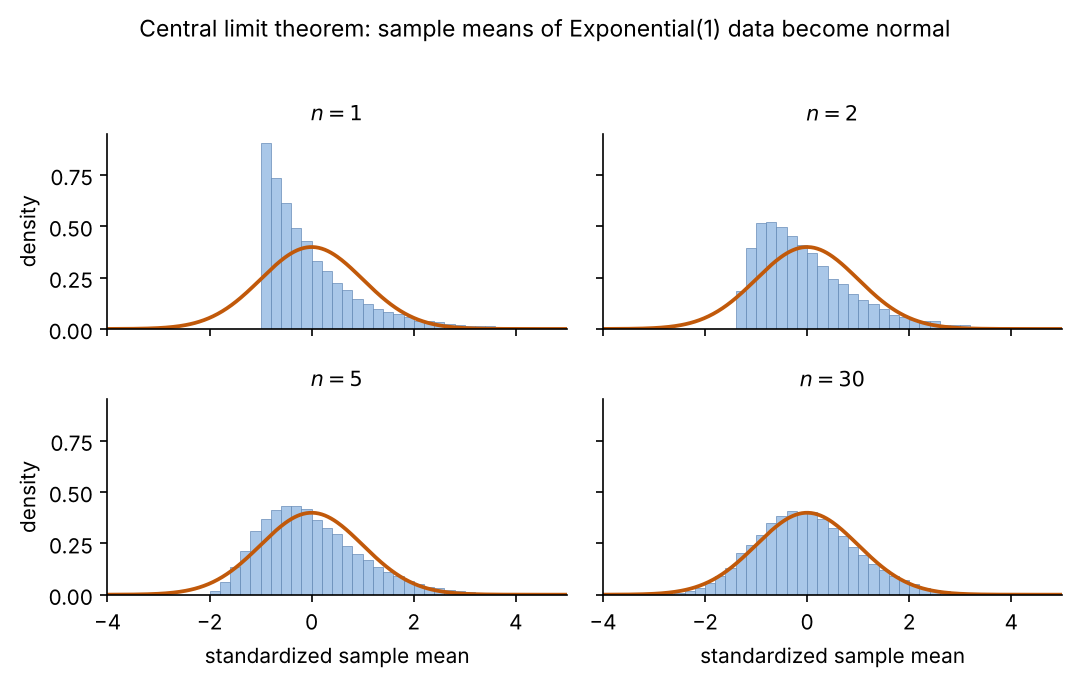
\includegraphics[width=\linewidth]{figures/clt_panel.png}
\end{figure}

\noindent At $n=1$ the standardized ``mean'' is just the raw
Exponential$(1)$, sharply right-skewed. By $n=5$ the skew is fading, and by
$n=30$ the histogram and the $N(0,1)$ curve are on top of each other. Nothing
about the exponential survives the averaging.

% ======================================================================
\section{Why they are true}
% ======================================================================

Both theorems come from controlling how much probability can sit far from the
mean. Two inequalities do all the work, and the first needs almost nothing.

\begin{theorem}[Markov's inequality]
If $Y \ge 0$ and $a > 0$, then $P(Y \ge a) \le E[Y]/a$.
\end{theorem}
\begin{proof}
Since $Y \ge 0$, we have $a\,\mathbf 1\{Y \ge a\} \le Y$ (the left side is
either $0$ or $a$, and when it is $a$ then $Y \ge a$). Taking expectations,
$a\,P(Y \ge a) \le E[Y]$, which rearranges to the claim.
\end{proof}

\begin{theorem}[Chebyshev's inequality]
For any random variable with mean $\mu$ and variance $\sigma^2$, and any
$\varepsilon > 0$,
\[
  P\big(|X - \mu| \ge \varepsilon\big) \le \frac{\sigma^2}{\varepsilon^2}.
\]
\end{theorem}
\begin{proof}
Apply Markov's inequality to the non-negative variable $Y = (X-\mu)^2$ with
$a = \varepsilon^2$:
\[
  P\big((X-\mu)^2 \ge \varepsilon^2\big)
    \le \frac{E[(X-\mu)^2]}{\varepsilon^2} = \frac{\sigma^2}{\varepsilon^2}.
\]
The event $(X-\mu)^2 \ge \varepsilon^2$ is the same as
$|X-\mu| \ge \varepsilon$.
\end{proof}

The weak law now falls out in one line.

\begin{proof}[Proof of the weak law of large numbers]
The sample mean has variance $\sigma^2/n$, so Chebyshev's inequality gives,
for any $\varepsilon > 0$,
\[
  P\big(|\bar X_n - \mu| \ge \varepsilon\big)
    \le \frac{\sigma^2/n}{\varepsilon^2}
    = \frac{\sigma^2}{n\,\varepsilon^2} \longrightarrow 0. \qedhere
\]
\end{proof}

The central limit theorem is deeper, but a clean proof runs through the
moment generating function.

\begin{theorem}[CLT via the MGF, sketch]
Standardize: let $Y_i = (X_i - \mu)/\sigma$, so $E[Y_i]=0$,
$\operatorname{Var}(Y_i)=1$, with MGF $m(t) = 1 + \tfrac{t^2}{2} + o(t^2)$.
Write $Z_n = \frac{1}{\sqrt n}\sum_{i=1}^n Y_i$. By independence,
\[
  M_{Z_n}(t) = \Big[\,m\!\big(t/\sqrt n\big)\Big]^{n}
             = \Big[\,1 + \frac{t^2}{2n} + o\!\big(1/n\big)\Big]^{n}
             \longrightarrow e^{t^2/2},
\]
which is the MGF of $N(0,1)$. Convergence of MGFs implies convergence in
distribution, so $Z_n \xrightarrow{d} N(0,1)$.
\end{theorem}

\noindent The limit $e^{t^2/2}$ depends only on the first two moments of the
$Y_i$ --- mean $0$ and variance $1$ --- which is exactly why every
finite-variance distribution lands on the same normal curve.

% ======================================================================
\section{Modes of convergence and the tools built on them}
% ======================================================================

We have used two modes of convergence; there are four worth naming, from
strongest to weakest. $Y_n \to Y$ \keyterm{almost surely} ($\xrightarrow{a.s.}$)
if $P(\lim_n Y_n = Y) = 1$; \keyterm{in mean square} if
$E|Y_n - Y|^2 \to 0$; \keyterm{in probability}; and \keyterm{in distribution}.
The implications go one way,
\[
  \xrightarrow{a.s.} \ \Longrightarrow\ \xrightarrow{p}\ \Longrightarrow\ \xrightarrow{d},
  \qquad
  \text{mean square} \ \Longrightarrow\ \xrightarrow{p},
\]
and none of the arrows reverses --- except that convergence in distribution
\emph{to a constant} does imply convergence in probability. (The ``weak'' in
the weak law is this distinction: the \emph{strong} law upgrades the same
conclusion to almost-sure convergence.)

Three tools let these limits be combined, and they are used constantly once
estimators get plugged into one another.

\begin{theorem}[Slutsky]
If $X_n \xrightarrow{d} X$ and $Y_n \xrightarrow{p} c$ for a constant $c$,
then $X_n + Y_n \xrightarrow{d} X + c$, \ $X_n Y_n \xrightarrow{d} cX$, and
$X_n / Y_n \xrightarrow{d} X/c$ \ (for $c \ne 0$).
\end{theorem}

This is what lets you replace an unknown $\sigma$ in
$\sqrt n(\bar X_n - \mu)/\sigma$ by a consistent estimate $\hat\sigma$ and
keep the same normal limit --- the basis of every $t$-statistic and
confidence interval.

\begin{theorem}[Continuous mapping]
If $g$ is continuous and $X_n \xrightarrow{d} X$, then
$g(X_n) \xrightarrow{d} g(X)$ (the same holds for $\xrightarrow{p}$ and
$\xrightarrow{a.s.}$).
\end{theorem}

\begin{theorem}[Delta method]
If $\sqrt n\,(\hat\theta - \theta) \xrightarrow{d} N(0,\sigma^2)$ and $g$ is
differentiable at $\theta$ with $g'(\theta) \ne 0$, then
\[
  \sqrt n\,\big(g(\hat\theta) - g(\theta)\big)
    \xrightarrow{d} N\!\big(0,\; g'(\theta)^2\,\sigma^2\big).
\]
\end{theorem}
\begin{proof}[Sketch]
A first-order Taylor expansion gives
$g(\hat\theta) = g(\theta) + g'(\theta)(\hat\theta - \theta) + R_n$, where the
remainder $R_n$ is negligible because $\hat\theta \xrightarrow{p} \theta$.
Multiplying by $\sqrt n$, the leading term is
$g'(\theta)\cdot\sqrt n(\hat\theta-\theta) \xrightarrow{d} g'(\theta)\,N(0,\sigma^2)
= N(0, g'(\theta)^2\sigma^2)$, and Slutsky absorbs the remainder.
\end{proof}

\noindent The delta method is how the asymptotic normality of an estimator
(for instance the maximum-likelihood estimator of Chapter 6) passes to any
smooth function of it. When the terms being summed are independent but
\emph{not} identically distributed --- weighted sums, regression residuals ---
the central limit theorem still holds under the \keyterm{Lindeberg condition},
which asks only that no single term contributes a non-vanishing share of the
total variance.

\begin{summarybox}
The sample mean converges to the truth (law of large numbers,
$\bar X_n \xrightarrow{p} \mu$) and its error is normal whatever the data
distribution (central limit theorem,
$\sqrt n(\bar X_n - \mu)\xrightarrow{d} N(0,\sigma^2)$). Both follow from
Markov's and Chebyshev's inequalities and the moment generating function.
Four modes of convergence (almost sure, mean square, probability,
distribution) are linked by one-way implications, and Slutsky's theorem, the
continuous mapping theorem and the delta method are the tools that carry
these limits through the estimators built in the rest of the course.
\end{summarybox}

\end{document}
